\section{Estandarización de procesos de trabajo}
Esta sección describe los procesos de trabajo que se
han identificado y como se han estandarizado. Se describen
los tres procesos principales que se han identificado dentro
del proyecto: integración de una integrante en el flujo de trabajo,
desarrollo de un proyecto desde cero y contribución al sistema
de conocimiento.

\subsection{Integración en el flujo de trabajo}
La integración de nuevas personas a un grupo de trabajo es fundamental
dentro de una empresa. Cuando se añaden nuevos miembros, es natural que 
surja cierta fricción debido a diversos factores, como la adaptación a 
la dinámica del equipo, la comprensión de los procesos establecidos y la 
familiarización con las herramientas y tecnologías utilizadas. Esta fricción 
puede ralentizar el progreso del equipo.\medskip

Una forma efectiva de mejorar esta cuestión es mediante la automatización de 
procesos, como la instalación y configuración de herramientas y software necesarios 
para el trabajo del equipo. Al utilizar un script que realiza estas tareas de 
forma automática, se eliminan los posibles errores humanos y se agiliza el proceso 
de integración de los nuevos miembros. Además, al estandarizar la configuración, 
se garantiza que todos los miembros del equipo tengan el mismo entorno de trabajo, 
lo que facilita la compatibilidad. Otro beneficio es que este script puede ser
también utilizado por miembros actuales del equipo para actualizar su entorno de
trabajo actual a las últimas versiones de las herramientas y software utilizados.

\subsubsection{Herramientas de desarrollo}
A continuación se describen las herramientas que se encuentran dentro del marco
de trabajo del equipo:
\begin{itemize}
    \item \textbf{Python3.11:} se ha elegido la versión 3.11 de Python como versión
    principal para el desarrollo de proyectos. La 3.11 ha traído mejoras significativas
    en cuanto a rendimiento y nuevas funcionalidades sobre la librería estándar como
    el módulo \textit{tomlib} que facilita de la lectura de los toml. Esta versión
    de python es el paquete del repositorio de DeadSnakes, no se utiliza conda ya
    que requiere de una licencia para su uso y no trae ventajas frente a la base.
    \item \textbf{Docker:} debido a que en la actualidad muchos proyectos han de funcionar
    dentro de contenedores, se ha decidido incluir Docker como una de las herramientas por
    dos razones, dar soporte a la virtualización de ciertos proyectos y facilitar su instalación
    que puede llegar a ser complicada si no se tiene experiencia previa.
    \item \textbf{Pipx:} es una herramienta que permite instalar otras herramientas de 
    consola de python de forma aislada, evitando así conflictos entre las distintas 
    versiones de las librerías.
    \item \textbf{Poetry:} es un gestor de dependencias y empaquetador de proyectos de python.
    Se ha incorporado ya que el desarrollo de componentes requiere de una forma sencilla de
    publicar y gestionar las dependencias de cada proyecto. Existe también alternativas como
    Pipenv, pero se ha preferido Poetry por que permite gestionar repositorios privados de una
    forma mas sencilla.  
    \item \textbf{Visual Studio Code:} 
    \item \textbf{Ruff:} es una herramienta que se encarga de corregir los errores de estilo
    y formatear el código fuente. Se ha elegido Ruff por encima de otras herramientas como
    Black o Flake8 debido a que Ruff ya combina las funcionalidades de ambas herramientas. Además,
    al estar escrita en rust es mucho más rápida que las otras herramientas. Se puede ver en la 
    figura \ref{fig:ruff-perfor} una comparativa de rendimiento \cite{astralRuff} sobre el repositorio de CPython.
    \begin{figure}[ht]
        \centering
        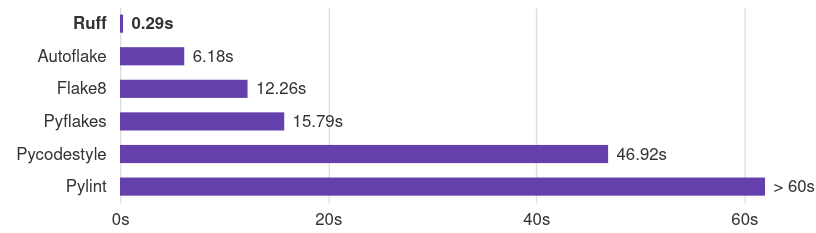
\includegraphics[width=0.8\textwidth]{ruff-perfor.png}
        \caption{Comparativa de rendimiento sobre el repositorio de CPython}\label{fig:ruff-perfor}
    \end{figure}
    \item \textbf{Cookiecutter:} 
\end{itemize}

\subsection{Desarrollo dentro de proyectos}
% Hablar aquí de las tres aportaciones que se han hecho Forecasting, 
\subsubsection{Puesta en practica de la metodología}
\subsection{Contribución al sistema de conocimiento}

\pagebreak
